% Created 2020-05-19 Tue 00:27
% Intended LaTeX compiler: pdflatex
\documentclass[11pt]{article}
\usepackage[utf8]{inputenc}
\usepackage[T1]{fontenc}
\usepackage{graphicx}
\usepackage{grffile}
\usepackage{longtable}
\usepackage{wrapfig}
\usepackage{rotating}
\usepackage[normalem]{ulem}
\usepackage{amsmath}
\usepackage{textcomp}
\usepackage{amssymb}
\usepackage{capt-of}
\usepackage{hyperref}
\usepackage{minted}
\usemintedstyle{native}
\author{mark}
\date{\today}
\title{UK.R}
\hypersetup{
 pdfauthor={mark},
 pdftitle={UK.R},
 pdfkeywords={},
 pdfsubject={},
 pdfcreator={Emacs 26.3 (Org mode 9.4)}, 
 pdflang={English}}
\begin{document}

\maketitle
\tableofcontents

-\textbf{- mode: org-mode; eval: (setq-local org-babel-default-header-args:R '((:session . ``R-session'') (:results . ``output org'') (:exports . ``both'') (:eval . ``never-export''))); -}-
Import some libraries:
\begin{minted}[bgColor=LightGray]{r}
library(rlang)
library(reshape2)
library(stringr)
library(rprojroot)
library(tibble)
\end{minted}

Some setup of directories, sourcing code and building:
\begin{minted}[bgColor=LightGray]{r}
covid_uk_path = getwd()
cm_path = file.path(covid_uk_path, "covidm");
source(file.path(cm_path, "R/covidm.R"))

\end{minted}

\section{Regions}
\label{sec:org4773db7}
\subsection{level 0}
\label{sec:org1c4a0f0}
Look for regions with different level/granularity:
\begin{minted}[bgColor=LightGray]{r}
cm_uk_locations("UK", 0)
\end{minted}

\begin{minted}[bgColor=LightGray]{org}
[1] "UK | UNITED KINGDOM"
\end{minted}

In this case, since ``level'' is zero, only fetch UK region.

We can do the same thing for regions of the UK at level 2
\subsection{level 1}
\label{sec:org0c9cb6b}
Look for regions with different level/granularity:
\begin{minted}[bgColor=LightGray]{r}
cm_uk_locations("UK", 1)
\end{minted}

\begin{minted}[bgColor=LightGray]{org}
[1] "UK | ENGLAND"          "UK | WALES"            "UK | SCOTLAND"         "UK | NORTHERN IRELAND"
\end{minted}

Wales is here as an aggregate region.

\subsection{level 2}
\label{sec:org6eb0a75}
\begin{minted}[bgColor=LightGray]{r}
locations = cm_uk_locations("UK", 2);
locations
\end{minted}

\begin{minted}[bgColor=LightGray]{org}

 [1] "UK | NORTH EAST"               "UK | NORTH WEST"               "UK | YORKSHIRE AND THE HUMBER" "UK | EAST MIDLANDS"            "UK | WEST MIDLANDS"            "UK | EAST"                     "UK | LONDON"                   "UK | SOUTH EAST"               "UK | SOUTH WEST"               "UK | WALES"                    "UK | SCOTLAND"                 "UK | NORTHERN IRELAND"
\end{minted}

\subsection{level 3}
\label{sec:org675250e}
\begin{minted}[bgColor=LightGray]{r}
locations = cm_uk_locations("UK", 3);
locations
\end{minted}

\begin{minted}[bgColor=LightGray]{org}

  [1] "UK | County Durham"                        "UK | Darlington"                           "UK | Hartlepool"                           "UK | Middlesbrough"                        "UK | Northumberland"                       "UK | Redcar and Cleveland"                 "UK | Stockton-on-Tees"                     "UK | Tyne and Wear (Met County)"           "UK | Blackburn with Darwen"                "UK | Blackpool"                            "UK | Cheshire East"                        "UK | Cheshire West and Chester"            "UK | Halton"                               "UK | Warrington"                           "UK | Cumbria"                              "UK | Greater Manchester (Met County)"      "UK | Lancashire"                           "UK | Merseyside (Met County)"              "UK | East Riding of Yorkshire"             "UK | Kingston upon Hull, City of"          "UK | North East Lincolnshire"              "UK | North Lincolnshire"                  
 [23] "UK | York"                                 "UK | North Yorkshire"                      "UK | South Yorkshire (Met County)"         "UK | West Yorkshire (Met County)"          "UK | Derby"                                "UK | Leicester"                            "UK | Nottingham"                           "UK | Rutland"                              "UK | Derbyshire"                           "UK | Leicestershire"                       "UK | Lincolnshire"                         "UK | Northamptonshire"                     "UK | Nottinghamshire"                      "UK | Herefordshire, County of"             "UK | Shropshire"                           "UK | Stoke-on-Trent"                       "UK | Telford and Wrekin"                   "UK | Staffordshire"                        "UK | Warwickshire"                         "UK | West Midlands (Met County)"           "UK | Worcestershire"                       "UK | Bedford"                             
 [45] "UK | Central Bedfordshire"                 "UK | Luton"                                "UK | Peterborough"                         "UK | Southend-on-Sea"                      "UK | Thurrock"                             "UK | Cambridgeshire"                       "UK | Essex"                                "UK | Hertfordshire"                        "UK | Norfolk"                              "UK | Suffolk"                              "UK | Camden"                               "UK | City of London"                       "UK | Hackney"                              "UK | Hammersmith and Fulham"               "UK | Haringey"                             "UK | Islington"                            "UK | Kensington and Chelsea"               "UK | Lambeth"                              "UK | Lewisham"                             "UK | Newham"                               "UK | Southwark"                            "UK | Tower Hamlets"                       
 [67] "UK | Wandsworth"                           "UK | Westminster"                          "UK | Barking and Dagenham"                 "UK | Barnet"                               "UK | Bexley"                               "UK | Brent"                                "UK | Bromley"                              "UK | Croydon"                              "UK | Ealing"                               "UK | Enfield"                              "UK | Greenwich"                            "UK | Harrow"                               "UK | Havering"                             "UK | Hillingdon"                           "UK | Hounslow"                             "UK | Kingston upon Thames"                 "UK | Merton"                               "UK | Redbridge"                            "UK | Richmond upon Thames"                 "UK | Sutton"                               "UK | Waltham Forest"                       "UK | Bracknell Forest"                    
 [89] "UK | Brighton and Hove"                    "UK | Isle of Wight"                        "UK | Medway"                               "UK | Milton Keynes"                        "UK | Portsmouth"                           "UK | Reading"                              "UK | Slough"                               "UK | Southampton"                          "UK | West Berkshire"                       "UK | Windsor and Maidenhead"               "UK | Wokingham"                            "UK | Buckinghamshire"                      "UK | East Sussex"                          "UK | Hampshire"                            "UK | Kent"                                 "UK | Oxfordshire"                          "UK | Surrey"                               "UK | West Sussex"                          "UK | Bath and North East Somerset"         "UK | Bournemouth, Christchurch and Poole"  "UK | Bristol, City of"                     "UK | Cornwall"                            
[111] "UK | Dorset"                               "UK | Isles of Scilly"                      "UK | North Somerset"                       "UK | Plymouth"                             "UK | South Gloucestershire"                "UK | Swindon"                              "UK | Torbay"                               "UK | Wiltshire"                            "UK | Devon"                                "UK | Gloucestershire"                      "UK | Somerset"                             "UK | Isle of Anglesey"                     "UK | Gwynedd"                              "UK | Conwy"                                "UK | Denbighshire"                         "UK | Flintshire"                           "UK | Wrexham"                              "UK | Powys"                                "UK | Ceredigion"                           "UK | Pembrokeshire"                        "UK | Carmarthenshire"                      "UK | Swansea"                             
[133] "UK | Neath Port Talbot"                    "UK | Bridgend"                             "UK | Vale of Glamorgan"                    "UK | Cardiff"                              "UK | Rhondda Cynon Taf"                    "UK | Merthyr Tydfil"                       "UK | Caerphilly"                           "UK | Blaenau Gwent"                        "UK | Torfaen"                              "UK | Monmouthshire"                        "UK | Newport"                              "UK | Aberdeen City"                        "UK | Aberdeenshire"                        "UK | Angus"                                "UK | Argyll and Bute"                      "UK | City of Edinburgh"                    "UK | Clackmannanshire"                     "UK | Dumfries and Galloway"                "UK | Dundee City"                          "UK | East Ayrshire"                        "UK | East Dunbartonshire"                  "UK | East Lothian"                        
[155] "UK | East Renfrewshire"                    "UK | Falkirk"                              "UK | Fife"                                 "UK | Glasgow City"                         "UK | Highland"                             "UK | Inverclyde"                           "UK | Midlothian"                           "UK | Moray"                                "UK | Na h-Eileanan Siar"                   "UK | North Ayrshire"                       "UK | North Lanarkshire"                    "UK | Orkney Islands"                       "UK | Perth and Kinross"                    "UK | Renfrewshire"                         "UK | Scottish Borders"                     "UK | Shetland Islands"                     "UK | South Ayrshire"                       "UK | South Lanarkshire"                    "UK | Stirling"                             "UK | West Dunbartonshire"                  "UK | West Lothian"                         "UK | Antrim and Newtownabbey"             
[177] "UK | Ards and North Down"                  "UK | Armagh City, Banbridge and Craigavon" "UK | Belfast"                              "UK | Causeway Coast and Glens"             "UK | Derry City and Strabane"              "UK | Fermanagh and Omagh"                  "UK | Lisburn and Castlereagh"              "UK | Mid and East Antrim"                  "UK | Mid Ulster"                           "UK | Newry, Mourne and Down"
\end{minted}

\subsection{level 4}
\label{sec:orgc5dd48f}
\begin{minted}[bgColor=LightGray]{r}
locations = cm_uk_locations("UK", 4);
locations
\end{minted}

\begin{minted}[bgColor=LightGray]{org}

  [1] "UK | County Durham"                        "UK | Darlington"                           "UK | Hartlepool"                           "UK | Middlesbrough"                        "UK | Northumberland"                       "UK | Redcar and Cleveland"                 "UK | Stockton-on-Tees"                     "UK | Gateshead"                            "UK | Newcastle upon Tyne"                  "UK | North Tyneside"                       "UK | South Tyneside"                       "UK | Sunderland"                           "UK | Blackburn with Darwen"                "UK | Blackpool"                            "UK | Cheshire East"                        "UK | Cheshire West and Chester"            "UK | Halton"                               "UK | Warrington"                           "UK | Allerdale"                            "UK | Barrow-in-Furness"                    "UK | Carlisle"                             "UK | Copeland"                            
 [23] "UK | Eden"                                 "UK | South Lakeland"                       "UK | Bolton"                               "UK | Bury"                                 "UK | Manchester"                           "UK | Oldham"                               "UK | Rochdale"                             "UK | Salford"                              "UK | Stockport"                            "UK | Tameside"                             "UK | Trafford"                             "UK | Wigan"                                "UK | Burnley"                              "UK | Chorley"                              "UK | Fylde"                                "UK | Hyndburn"                             "UK | Lancaster"                            "UK | Pendle"                               "UK | Preston"                              "UK | Ribble Valley"                        "UK | Rossendale"                           "UK | South Ribble"                        
 [45] "UK | West Lancashire"                      "UK | Wyre"                                 "UK | Knowsley"                             "UK | Liverpool"                            "UK | Sefton"                               "UK | St. Helens"                           "UK | Wirral"                               "UK | East Riding of Yorkshire"             "UK | Kingston upon Hull, City of"          "UK | North East Lincolnshire"              "UK | North Lincolnshire"                   "UK | York"                                 "UK | Craven"                               "UK | Hambleton"                            "UK | Harrogate"                            "UK | Richmondshire"                        "UK | Ryedale"                              "UK | Scarborough"                          "UK | Selby"                                "UK | Barnsley"                             "UK | Doncaster"                            "UK | Rotherham"                           
 [67] "UK | Sheffield"                            "UK | Bradford"                             "UK | Calderdale"                           "UK | Kirklees"                             "UK | Leeds"                                "UK | Wakefield"                            "UK | Derby"                                "UK | Leicester"                            "UK | Nottingham"                           "UK | Rutland"                              "UK | Amber Valley"                         "UK | Bolsover"                             "UK | Chesterfield"                         "UK | Derbyshire Dales"                     "UK | Erewash"                              "UK | High Peak"                            "UK | North East Derbyshire"                "UK | South Derbyshire"                     "UK | Blaby"                                "UK | Charnwood"                            "UK | Harborough"                           "UK | Hinckley and Bosworth"               
 [89] "UK | Melton"                               "UK | North West Leicestershire"            "UK | Oadby and Wigston"                    "UK | Boston"                               "UK | East Lindsey"                         "UK | Lincoln"                              "UK | North Kesteven"                       "UK | South Holland"                        "UK | South Kesteven"                       "UK | West Lindsey"                         "UK | Corby"                                "UK | Daventry"                             "UK | East Northamptonshire"                "UK | Kettering"                            "UK | Northampton"                          "UK | South Northamptonshire"               "UK | Wellingborough"                       "UK | Ashfield"                             "UK | Bassetlaw"                            "UK | Broxtowe"                             "UK | Gedling"                              "UK | Mansfield"                           
[111] "UK | Newark and Sherwood"                  "UK | Rushcliffe"                           "UK | Herefordshire, County of"             "UK | Shropshire"                           "UK | Stoke-on-Trent"                       "UK | Telford and Wrekin"                   "UK | Cannock Chase"                        "UK | East Staffordshire"                   "UK | Lichfield"                            "UK | Newcastle-under-Lyme"                 "UK | South Staffordshire"                  "UK | Stafford"                             "UK | Staffordshire Moorlands"              "UK | Tamworth"                             "UK | North Warwickshire"                   "UK | Nuneaton and Bedworth"                "UK | Rugby"                                "UK | Stratford-on-Avon"                    "UK | Warwick"                              "UK | Birmingham"                           "UK | Coventry"                             "UK | Dudley"                              
[133] "UK | Sandwell"                             "UK | Solihull"                             "UK | Walsall"                              "UK | Wolverhampton"                        "UK | Bromsgrove"                           "UK | Malvern Hills"                        "UK | Redditch"                             "UK | Worcester"                            "UK | Wychavon"                             "UK | Wyre Forest"                          "UK | Bedford"                              "UK | Central Bedfordshire"                 "UK | Luton"                                "UK | Peterborough"                         "UK | Southend-on-Sea"                      "UK | Thurrock"                             "UK | Cambridge"                            "UK | East Cambridgeshire"                  "UK | Fenland"                              "UK | Huntingdonshire"                      "UK | South Cambridgeshire"                 "UK | Basildon"                            
[155] "UK | Braintree"                            "UK | Brentwood"                            "UK | Castle Point"                         "UK | Chelmsford"                           "UK | Colchester"                           "UK | Epping Forest"                        "UK | Harlow"                               "UK | Maldon"                               "UK | Rochford"                             "UK | Tendring"                             "UK | Uttlesford"                           "UK | Broxbourne"                           "UK | Dacorum"                              "UK | East Hertfordshire"                   "UK | Hertsmere"                            "UK | North Hertfordshire"                  "UK | St Albans"                            "UK | Stevenage"                            "UK | Three Rivers"                         "UK | Watford"                              "UK | Welwyn Hatfield"                      "UK | Breckland"                           
[177] "UK | Broadland"                            "UK | Great Yarmouth"                       "UK | King's Lynn and West Norfolk"         "UK | North Norfolk"                        "UK | Norwich"                              "UK | South Norfolk"                        "UK | Babergh"                              "UK | East Suffolk"                         "UK | Ipswich"                              "UK | Mid Suffolk"                          "UK | West Suffolk"                         "UK | Camden"                               "UK | City of London"                       "UK | Hackney"                              "UK | Hammersmith and Fulham"               "UK | Haringey"                             "UK | Islington"                            "UK | Kensington and Chelsea"               "UK | Lambeth"                              "UK | Lewisham"                             "UK | Newham"                               "UK | Southwark"                           
[199] "UK | Tower Hamlets"                        "UK | Wandsworth"                           "UK | Westminster"                          "UK | Barking and Dagenham"                 "UK | Barnet"                               "UK | Bexley"                               "UK | Brent"                                "UK | Bromley"                              "UK | Croydon"                              "UK | Ealing"                               "UK | Enfield"                              "UK | Greenwich"                            "UK | Harrow"                               "UK | Havering"                             "UK | Hillingdon"                           "UK | Hounslow"                             "UK | Kingston upon Thames"                 "UK | Merton"                               "UK | Redbridge"                            "UK | Richmond upon Thames"                 "UK | Sutton"                               "UK | Waltham Forest"                      
[221] "UK | Bracknell Forest"                     "UK | Brighton and Hove"                    "UK | Isle of Wight"                        "UK | Medway"                               "UK | Milton Keynes"                        "UK | Portsmouth"                           "UK | Reading"                              "UK | Slough"                               "UK | Southampton"                          "UK | West Berkshire"                       "UK | Windsor and Maidenhead"               "UK | Wokingham"                            "UK | Aylesbury Vale"                       "UK | Chiltern"                             "UK | South Bucks"                          "UK | Wycombe"                              "UK | Eastbourne"                           "UK | Hastings"                             "UK | Lewes"                                "UK | Rother"                               "UK | Wealden"                              "UK | Basingstoke and Deane"               
[243] "UK | East Hampshire"                       "UK | Eastleigh"                            "UK | Fareham"                              "UK | Gosport"                              "UK | Hart"                                 "UK | Havant"                               "UK | New Forest"                           "UK | Rushmoor"                             "UK | Test Valley"                          "UK | Winchester"                           "UK | Ashford"                              "UK | Canterbury"                           "UK | Dartford"                             "UK | Dover"                                "UK | Folkestone and Hythe"                 "UK | Gravesham"                            "UK | Maidstone"                            "UK | Sevenoaks"                            "UK | Swale"                                "UK | Thanet"                               "UK | Tonbridge and Malling"                "UK | Tunbridge Wells"                     
[265] "UK | Cherwell"                             "UK | Oxford"                               "UK | South Oxfordshire"                    "UK | Vale of White Horse"                  "UK | West Oxfordshire"                     "UK | Elmbridge"                            "UK | Epsom and Ewell"                      "UK | Guildford"                            "UK | Mole Valley"                          "UK | Reigate and Banstead"                 "UK | Runnymede"                            "UK | Spelthorne"                           "UK | Surrey Heath"                         "UK | Tandridge"                            "UK | Waverley"                             "UK | Woking"                               "UK | Adur"                                 "UK | Arun"                                 "UK | Chichester"                           "UK | Crawley"                              "UK | Horsham"                              "UK | Mid Sussex"                          
[287] "UK | Worthing"                             "UK | Bath and North East Somerset"         "UK | Bournemouth, Christchurch and Poole"  "UK | Bristol, City of"                     "UK | Cornwall"                             "UK | Dorset"                               "UK | Isles of Scilly"                      "UK | North Somerset"                       "UK | Plymouth"                             "UK | South Gloucestershire"                "UK | Swindon"                              "UK | Torbay"                               "UK | Wiltshire"                            "UK | East Devon"                           "UK | Exeter"                               "UK | Mid Devon"                            "UK | North Devon"                          "UK | South Hams"                           "UK | Teignbridge"                          "UK | Torridge"                             "UK | West Devon"                           "UK | Cheltenham"                          
[309] "UK | Cotswold"                             "UK | Forest of Dean"                       "UK | Gloucester"                           "UK | Stroud"                               "UK | Tewkesbury"                           "UK | Mendip"                               "UK | Sedgemoor"                            "UK | Somerset West and Taunton"            "UK | South Somerset"                       "UK | Isle of Anglesey"                     "UK | Gwynedd"                              "UK | Conwy"                                "UK | Denbighshire"                         "UK | Flintshire"                           "UK | Wrexham"                              "UK | Powys"                                "UK | Ceredigion"                           "UK | Pembrokeshire"                        "UK | Carmarthenshire"                      "UK | Swansea"                              "UK | Neath Port Talbot"                    "UK | Bridgend"                            
[331] "UK | Vale of Glamorgan"                    "UK | Cardiff"                              "UK | Rhondda Cynon Taf"                    "UK | Merthyr Tydfil"                       "UK | Caerphilly"                           "UK | Blaenau Gwent"                        "UK | Torfaen"                              "UK | Monmouthshire"                        "UK | Newport"                              "UK | Aberdeen City"                        "UK | Aberdeenshire"                        "UK | Angus"                                "UK | Argyll and Bute"                      "UK | City of Edinburgh"                    "UK | Clackmannanshire"                     "UK | Dumfries and Galloway"                "UK | Dundee City"                          "UK | East Ayrshire"                        "UK | East Dunbartonshire"                  "UK | East Lothian"                         "UK | East Renfrewshire"                    "UK | Falkirk"                             
[353] "UK | Fife"                                 "UK | Glasgow City"                         "UK | Highland"                             "UK | Inverclyde"                           "UK | Midlothian"                           "UK | Moray"                                "UK | Na h-Eileanan Siar"                   "UK | North Ayrshire"                       "UK | North Lanarkshire"                    "UK | Orkney Islands"                       "UK | Perth and Kinross"                    "UK | Renfrewshire"                         "UK | Scottish Borders"                     "UK | Shetland Islands"                     "UK | South Ayrshire"                       "UK | South Lanarkshire"                    "UK | Stirling"                             "UK | West Dunbartonshire"                  "UK | West Lothian"                         "UK | Antrim and Newtownabbey"              "UK | Ards and North Down"                  "UK | Armagh City, Banbridge and Craigavon"
[375] "UK | Belfast"                              "UK | Causeway Coast and Glens"             "UK | Derry City and Strabane"              "UK | Fermanagh and Omagh"                  "UK | Lisburn and Castlereagh"              "UK | Mid and East Antrim"                  "UK | Mid Ulster"                           "UK | Newry, Mourne and Down"
\end{minted}

\section{UK Parameters}
\label{sec:org7c7a62c}
Build parameters:
\begin{minted}[bgColor=LightGray]{r}
parametersUK1 = cm_parameters_SEI3R(cm_uk_locations("UK", 0),
    dE  = cm_delay_gamma(4.0, 4.0, t_max = 60, t_step = 0.25)$p,
    dIp = cm_delay_gamma(1.5, 4.0, t_max = 60, t_step = 0.25)$p,
    dIs = cm_delay_gamma(3.5, 4.0, t_max = 60, t_step = 0.25)$p,
    dIa = cm_delay_gamma(5.0, 4.0, t_max = 60, t_step = 0.25)$p,
    deterministic = F);
\end{minted}

Comments, from further down the script, on the same parameters:
dE  = \# 6.5 day serial interval.
dIp = \# 1.5 days w/o symptoms
dIs = \# 5 days total of infectiousness
dIa = \# 5 days total of infectiousness here as well.

\begin{minted}[bgColor=LightGray]{r}
show_fields <- function (p, ...) {
disp_names <- list(...)
str <- Reduce(function (str, index) { paste0(str, " ", index, " : ", p[index], "\n") }, disp_names, "")
}

print_params <- function(params, npops) {
  paste0("Duration fields:\n",
         show_fields(params, "date0", "time0", "time1", "time_step"),
         "\n\nBehavioural flag fields\n",
         show_fields("report_every", "fast_multinomial", "deterministric"),
         "\n\nPopulations [", length(params$pop), "]:\n",
         paste(lapply(params$pop[1:npops], "[[", "name"), collapse="\n"),
         ifelse(npops < length(params$pop), " ...", "")
         )
}
\end{minted}

\begin{minted}[bgColor=LightGray]{r}
print_params(parametersUK1, 1)
\end{minted}

\begin{minted}[bgColor=LightGray]{org}
Duration fields:
 date0 : 2020-03-01
 time0 : 0
 time1 : 2021-03-01
 time_step : 0.25


Behavioural flag fields
 fast_multinomial : NA
 deterministric : NA


Populations [1]:
UK | UNITED KINGDOM
\end{minted}

\begin{minted}[bgColor=LightGray]{org}
  type           : chr "SEI3R"
  dE             : num [1:241] 9.21e-06 6.02e-04 3.27e-03 8.38e-03 1.54e-02 ...
  dIp            : num [1:241] 0.000395 0.018594 0.069279 0.119197 0.145304 ...
  dIa            : num [1:241] 3.85e-06 2.62e-04 1.49e-03 4.00e-03 7.71e-03 ...
  dIs            : num [1:241] 1.55e-05 9.85e-04 5.17e-03 1.28e-02 2.27e-02 ...
  dH             : num 1
  dC             : num 1
  size           : num [1:16] 3914028 4138524 3858894 3669250 4184575 ...
  matrices       :List of 4
  contact        : num [1:4] 1 1 1 1
  contact_mult   : num(0) 
  contact_lowerto: num(0) 
  u              : num [1:16] 0.08 0.08 0.08 0.08 0.08 0.08 0.08 0.08 0.08 0.08 ...
  y              : num [1:16] 0.5 0.5 0.5 0.5 0.5 0.5 0.5 0.5 0.5 0.5 ...
  fIp            : num [1:16] 1 1 1 1 1 1 1 1 1 1 ...
  fIs            : num [1:16] 1 1 1 1 1 1 1 1 1 1 ...
  fIa            : num [1:16] 0.5 0.5 0.5 0.5 0.5 0.5 0.5 0.5 0.5 0.5 ...
  rho            : num [1:16] 1 1 1 1 1 1 1 1 1 1 ...
  tau            : num [1:16] 1 1 1 1 1 1 1 1 1 1 ...
  seed_times     : num 1
  dist_seed_ages : num [1:16] 1 1 1 1 1 1 1 1 1 1 ...
  schedule       : list()
  observer       : NULL
  name           : chr "UK | UNITED KINGDOM"
  group_names    : chr [1:16] "0-4" "5-9" "10-14" "15-19" ...
\end{minted}

\begin{minted}[bgColor=LightGray]{r}
library(RColorBrewer)

plot_matrices <- function(population, filters) {
    if(is.null(population$matrices)) {
        stop("No 'matrices' field. Are you passing a population rather than params?");
    }
    if(missing(filters)) {
        filters <- names(population$matrices)
    }
    
    dt <- melt(population$matrices[filters])

    # set first two columns to be x and y
    names(dt)[1] <- "x"
    names(dt)[2] <- "y"

    ggplot(data = dt, aes(x=x, y=y, fill=value)) + geom_tile() + facet_wrap(. ~ L1) + labs(title=population$name) +  scale_fill_gradient(low="white", high="blue")
} 
\end{minted}

Contact Matrices:
\begin{center}
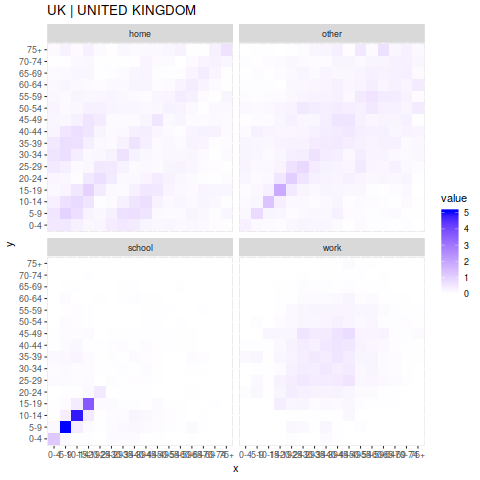
\includegraphics[width=.9\linewidth]{1-home.png}
\end{center}

The parameters for a ``generic'' simulation.

\begin{itemize}
\item date0, time0, time1 : time range of simulation (note: time1 is a date)
\item time\textsubscript{step} : steps to take (presumably in the simulation units, which are days)
\item report\textsubscript{every} - appears to record or set every report\textsubscript{every} timesteps
\item fast\textsubscript{multinomial} : choose which implementation of multinomail solution to use
\item deterministric : skips some seeding in time marching.
\item pop: populations, just one population (whole UK) in this case

\begin{minted}[bgColor=LightGray]{r}
matrix_summary <- function (matrices) {
ns <- names(matrices)
for (name in ns) {
print(name)
print(summary(parametersUK1$pop[[1]]$matrices[[name]]))
print("-------------------------------------------------------------------------")
}
}
\end{minted}

\begin{minted}[bgColor=LightGray]{r}
matrix_summary(parametersUK1$pop[[1]]$matrices)
\end{minted}

\begin{minted}[bgColor=LightGray]{org}
 [1] "home"
       0-4              5-9              10-14             15-19            20-24             25-29             30-34             35-39             40-44             45-49             50-54             55-59             60-64             65-69             70-74

  Min.   :0.0544   Min.   :0.05793   Min.   :0.06102   Min.   :0.1091   Min.   :0.03363   Min.   :0.01391   Min.   :0.02288   Min.   :0.06115   Min.   :0.07232   Min.   :0.09259   Min.   :0.04746   Min.   :0.01223   Min.   :0.02017   Min.   :0.01140   Min.   :0.009259   Min.   :0.01695  
  1st Qu.:0.1621   1st Qu.:0.16038   1st Qu.:0.15109   1st Qu.:0.1557   1st Qu.:0.10215   1st Qu.:0.11785   1st Qu.:0.14453   1st Qu.:0.12816   1st Qu.:0.14598   1st Qu.:0.11999   1st Qu.:0.15631   1st Qu.:0.11726   1st Qu.:0.11943   1st Qu.:0.06594   1st Qu.:0.044178   1st Qu.:0.10271  
  Median :0.1938   Median :0.24352   Median :0.23989   Median :0.2279   Median :0.17053   Median :0.18279   Median :0.17433   Median :0.24596   Median :0.22837   Median :0.16648   Median :0.17679   Median :0.18131   Median :0.15578   Median :0.12663   Median :0.108972   Median :0.15005  
  Mean   :0.2587   Mean   :0.36008   Mean   :0.32720   Mean   :0.3093   Mean   :0.23209   Mean   :0.22059   Mean   :0.26362   Mean   :0.29457   Mean   :0.27971   Mean   :0.22727   Mean   :0.19393   Mean   :0.18164   Mean   :0.17016   Mean   :0.14736   Mean   :0.111984   Mean   :0.18364  
  3rd Qu.:0.4050   3rd Qu.:0.57309   3rd Qu.:0.55518   3rd Qu.:0.4369   3rd Qu.:0.30889   3rd Qu.:0.30373   3rd Qu.:0.30886   3rd Qu.:0.38098   3rd Qu.:0.32694   3rd Qu.:0.24610   3rd Qu.:0.23691   3rd Qu.:0.22714   3rd Qu.:0.21386   3rd Qu.:0.21554   3rd Qu.:0.179548   3rd Qu.:0.27244  
  Max.   :0.4993   Max.   :0.94118   Max.   :0.80392   Max.   :0.9619   Max.   :0.69492   Max.   :0.47359   Max.   :0.68793   Max.   :0.70084   Max.   :0.68146   Max.   :0.57527   Max.   :0.31325   Max.   :0.38889   Max.   :0.40909   Max.   :0.40741   Max.   :0.272727   Max.   :0.62500  
 [1] "-------------------------------------------------------------------------"
 [1] "work"
       0-4                5-9               10-14             15-19              20-24             25-29              30-34             35-39             40-44             45-49             50-54             55-59             60-64             65-69             70-74

  Min.   :0.000000   Min.   :0.000000   Min.   :0.00000   Min.   :0.000000   Min.   :0.00000   Min.   :0.006953   Min.   :0.00000   Min.   :0.01619   Min.   :0.02335   Min.   :0.00000   Min.   :0.00000   Min.   :0.00000   Min.   :0.00000   Min.   :0.00000   Min.   :0.000000   Min.   :0.000000  
  1st Qu.:0.000000   1st Qu.:0.000000   1st Qu.:0.00000   1st Qu.:0.007676   1st Qu.:0.04926   1st Qu.:0.093358   1st Qu.:0.03803   1st Qu.:0.10946   1st Qu.:0.04798   1st Qu.:0.09051   1st Qu.:0.05703   1st Qu.:0.03008   1st Qu.:0.01406   1st Qu.:0.00000   1st Qu.:0.000000   1st Qu.:0.000000  
  Median :0.000000   Median :0.009307   Median :0.00920   Median :0.058526   Median :0.15692   Median :0.194046   Median :0.15411   Median :0.20479   Median :0.17892   Median :0.21845   Median :0.11323   Median :0.13525   Median :0.04557   Median :0.04114   Median :0.006548   Median :0.002381  
  Mean   :0.015903   Mean   :0.042219   Mean   :0.02083   Mean   :0.094666   Mean   :0.16089   Mean   :0.236826   Mean   :0.19564   Mean   :0.22977   Mean   :0.22198   Mean   :0.27043   Mean   :0.12480   Mean   :0.12076   Mean   :0.06549   Mean   :0.03224   Mean   :0.014003   Mean   :0.016386  
  3rd Qu.:0.008671   3rd Qu.:0.049204   3rd Qu.:0.01907   3rd Qu.:0.158738   3rd Qu.:0.26026   3rd Qu.:0.381874   3rd Qu.:0.36794   3rd Qu.:0.37314   3rd Qu.:0.34436   3rd Qu.:0.42546   3rd Qu.:0.19197   3rd Qu.:0.20630   3rd Qu.:0.10810   3rd Qu.:0.05354   3rd Qu.:0.029493   3rd Qu.:0.018506  
  Max.   :0.121429   Max.   :0.185714   Max.   :0.17273   Max.   :0.361905   Max.   :0.40678   Max.   :0.573534   Max.   :0.49164   Max.   :0.53276   Max.   :0.56452   Max.   :0.72727   Max.   :0.29591   Max.   :0.23231   Max.   :0.21302   Max.   :0.07863   Max.   :0.045455   Max.   :0.118182  
 [1] "-------------------------------------------------------------------------"
 [1] "school"
       0-4                5-9              10-14             15-19             20-24              25-29             30-34             35-39             40-44             45-49             50-54              55-59              60-64              65-69              70-74

  Min.   :0.000000   Min.   :0.00000   Min.   :0.00000   Min.   :0.00000   Min.   :0.000000   Min.   :0.00000   Min.   :0.00000   Min.   :0.00000   Min.   :0.00000   Min.   :0.00000   Min.   :0.000000   Min.   :0.000000   Min.   :0.000000   Min.   :0.000000   Min.   :0.000000   Min.   :0.000000  
  1st Qu.:0.008528   1st Qu.:0.04234   1st Qu.:0.02211   1st Qu.:0.02790   1st Qu.:0.007859   1st Qu.:0.00000   1st Qu.:0.02199   1st Qu.:0.02089   1st Qu.:0.02066   1st Qu.:0.01483   1st Qu.:0.000000   1st Qu.:0.007468   1st Qu.:0.000000   1st Qu.:0.000000   1st Qu.:0.000000   1st Qu.:0.000000  
  Median :0.024145   Median :0.09194   Median :0.06640   Median :0.05430   Median :0.012839   Median :0.02570   Median :0.04116   Median :0.05501   Median :0.04768   Median :0.02654   Median :0.003967   Median :0.009470   Median :0.009664   Median :0.002632   Median :0.000000   Median :0.000000  
  Mean   :0.112839   Mean   :0.41307   Mean   :0.40616   Mean   :0.30059   Mean   :0.052988   Mean   :0.04336   Mean   :0.05077   Mean   :0.06919   Mean   :0.05170   Mean   :0.03556   Mean   :0.020361   Mean   :0.018743   Mean   :0.017827   Mean   :0.011193   Mean   :0.002846   Mean   :0.000504  
  3rd Qu.:0.087690   3rd Qu.:0.14577   3rd Qu.:0.18155   3rd Qu.:0.09666   3rd Qu.:0.034847   3rd Qu.:0.07518   3rd Qu.:0.07962   3rd Qu.:0.09134   3rd Qu.:0.06546   3rd Qu.:0.03676   3rd Qu.:0.036908   3rd Qu.:0.034259   3rd Qu.:0.015812   3rd Qu.:0.024143   3rd Qu.:0.000000   3rd Qu.:0.000000  
  Max.   :1.178947   Max.   :5.07843   Max.   :4.87255   Max.   :3.64762   Max.   :0.457627   Max.   :0.11905   Max.   :0.15687   Max.   :0.24145   Max.   :0.17700   Max.   :0.11939   Max.   :0.078431   Max.   :0.054420   Max.   :0.088104   Max.   :0.043057   Max.   :0.040281   Max.   :0.008065  
 [1] "-------------------------------------------------------------------------"
 [1] "other"
       0-4                5-9              10-14             15-19              20-24             25-29             30-34            35-39            40-44            45-49             50-54            55-59             60-64             65-69             70-74

  Min.   :0.003734   Min.   :0.01838   Min.   :0.02743   Min.   :0.006333   Min.   :0.03214   Min.   :0.07838   Min.   :0.1021   Min.   :0.1127   Min.   :0.1316   Min.   :0.04211   Min.   :0.1029   Min.   :0.06784   Min.   :0.05326   Min.   :0.03591   Min.   :0.03746   Min.   :0.005263  
  1st Qu.:0.068520   1st Qu.:0.07807   1st Qu.:0.07448   1st Qu.:0.087384   1st Qu.:0.18017   1st Qu.:0.19131   1st Qu.:0.1770   1st Qu.:0.2123   1st Qu.:0.2214   1st Qu.:0.15844   1st Qu.:0.2263   1st Qu.:0.09159   1st Qu.:0.14142   1st Qu.:0.10682   1st Qu.:0.08358   1st Qu.:0.041584  
  Median :0.117469   Median :0.12445   Median :0.12179   Median :0.171740   Median :0.21659   Median :0.25651   Median :0.2330   Median :0.2771   Median :0.2797   Median :0.20970   Median :0.3227   Median :0.23708   Median :0.20947   Median :0.16465   Median :0.15730   Median :0.131614  
  Mean   :0.123138   Mean   :0.16894   Mean   :0.19769   Mean   :0.271905   Mean   :0.29216   Mean   :0.30281   Mean   :0.2674   Mean   :0.2795   Mean   :0.2858   Mean   :0.24544   Mean   :0.3068   Mean   :0.24723   Mean   :0.20887   Mean   :0.18300   Mean   :0.16215   Mean   :0.183660  
  3rd Qu.:0.177872   3rd Qu.:0.18420   3rd Qu.:0.15691   3rd Qu.:0.213914   3rd Qu.:0.30376   3rd Qu.:0.33748   3rd Qu.:0.3518   3rd Qu.:0.3338   3rd Qu.:0.3213   3rd Qu.:0.32408   3rd Qu.:0.3965   3rd Qu.:0.34283   3rd Qu.:0.26548   3rd Qu.:0.25302   3rd Qu.:0.21422   3rd Qu.:0.246897  
  Max.   :0.294737   Max.   :0.75490   Max.   :1.27451   Max.   :1.828571   Max.   :1.03390   Max.   :0.81356   Max.   :0.6167   Max.   :0.4438   Max.   :0.4864   Max.   :0.56364   Max.   :0.4799   Max.   :0.57407   Max.   :0.42775   Max.   :0.34672   Max.   :0.33193   Max.   :0.642539  
 [1] "-------------------------------------------------------------------------"
\end{minted}
\end{itemize}

\begin{minted}[bgColor=LightGray]{r}
more_than_val_summary <- function (population, label, val) {
   m <- population$matrices[[label]]
   idx <- which(m > val, arr.ind = T)
   out <- paste0(label, ":\n")
   if(length(idx) > 0 ) {
      out <- paste0(out,str_pad("i", 10, side="right"),str_pad("j",10,side="right"), "value", "\n")
      out <- paste0(out, "-------------------------------------\n")
      for (i in 1:nrow(idx)) {
          rname <- rownames(m)[idx[i,][1]]
          cname <- colnames(m)[idx[i,][2]]
          val <- m[idx[i,1], idx[i,2]]
          out <- paste0(out, str_pad(rname, 10, side="right"),str_pad(cname,10,side="right"), val, "\n")
      }
   } else {
      out <- paste0(out, "max = ", max(m))
   }
   out <- paste0(out, "\n\n")
}

summary_all_matrices_over_val <- function(population, val) {
out <- ""
for (i in names(parametersUK1$pop[[1]]$matrices)) {
  out <- paste0(out, more_than_val_summary(parametersUK1$pop[[1]], i, val))
}
out
}
\end{minted}

Values greater than 1:
\begin{minted}[bgColor=LightGray]{org}
home:
max = 0.961904761904762

work:
max = 0.727272727272727

school:
i         j         value
-------------------------------------
0-4       0-4       1.17894736842105
5-9       5-9       5.07843137254902
10-14     10-14     4.87254901960784
15-19     15-19     3.64761904761905


other:
i         j         value
-------------------------------------
10-14     10-14     1.27450980392157
15-19     15-19     1.82857142857143
20-24     20-24     1.03389830508475
\end{minted}

\section{UK Regions}
\label{sec:orge342611}
\subsection{Regional parameter setup}
\label{sec:orgfbdf340}
Set up regional parameters, down to county level (level = 3)
\begin{minted}[bgColor=LightGray]{r}
locations = cm_uk_locations("UK", 3);
parameters = cm_parameters_SEI3R(locations, date_start = "2020-01-29", date_end = "2021-12-31",
    dE  = cm_delay_gamma(4.0, 4.0, t_max = 60, t_step = 0.25)$p, # 6.5 day serial interval.
    dIp = cm_delay_gamma(1.5, 4.0, t_max = 60, t_step = 0.25)$p, # 1.5 days w/o symptoms
    dIs = cm_delay_gamma(3.5, 4.0, t_max = 60, t_step = 0.25)$p, # 5 days total of infectiousness
    dIa = cm_delay_gamma(5.0, 4.0, t_max = 60, t_step = 0.25)$p, # 5 days total of infectiousness here as well.
    deterministic = F);
\end{minted}

\begin{minted}[bgColor=LightGray]{r}
print_params(parameters, 10)
\end{minted}

\begin{minted}[bgColor=LightGray]{org}
Duration fields:
 date0 : 2020-01-29
 time0 : 0
 time1 : 2021-12-31
 time_step : 0.25


Behavioural flag fields
 fast_multinomial : NA
 deterministric : NA


Populations [186]:
UK | County Durham
UK | Darlington
UK | Hartlepool
UK | Middlesbrough
UK | Northumberland
UK | Redcar and Cleveland
UK | Stockton-on-Tees
UK | Tyne and Wear (Met County)
UK | Blackburn with Darwen
UK | Blackpool ...
\end{minted}

186 populations (one for each region at level 3).

Fields for first population:
\begin{minted}[bgColor=LightGray]{org}
  type           : chr "SEI3R"
  dE             : num [1:241] 9.21e-06 6.02e-04 3.27e-03 8.38e-03 1.54e-02 ...
  dIp            : num [1:241] 0.000395 0.018594 0.069279 0.119197 0.145304 ...
  dIa            : num [1:241] 3.85e-06 2.62e-04 1.49e-03 4.00e-03 7.71e-03 ...
  dIs            : num [1:241] 1.55e-05 9.85e-04 5.17e-03 1.28e-02 2.27e-02 ...
  dH             : num 1
  dC             : num 1
  size           : num [1:16] 27021 29989 28558 29134 35874 ...
  matrices       :List of 4
  contact        : num [1:4] 1 1 1 1
  contact_mult   : num(0) 
  contact_lowerto: num(0) 
  u              : num [1:16] 0.08 0.08 0.08 0.08 0.08 0.08 0.08 0.08 0.08 0.08 ...
  y              : num [1:16] 0.5 0.5 0.5 0.5 0.5 0.5 0.5 0.5 0.5 0.5 ...
  fIp            : num [1:16] 1 1 1 1 1 1 1 1 1 1 ...
  fIs            : num [1:16] 1 1 1 1 1 1 1 1 1 1 ...
  fIa            : num [1:16] 0.5 0.5 0.5 0.5 0.5 0.5 0.5 0.5 0.5 0.5 ...
  rho            : num [1:16] 1 1 1 1 1 1 1 1 1 1 ...
  tau            : num [1:16] 1 1 1 1 1 1 1 1 1 1 ...
  seed_times     : num 1
  dist_seed_ages : num [1:16] 1 1 1 1 1 1 1 1 1 1 ...
  schedule       : list()
  observer       : NULL
  name           : chr "UK | County Durham"
  group_names    : chr [1:16] "0-4" "5-9" "10-14" "15-19" ...
\end{minted}

Matrices for first population:
\begin{center}
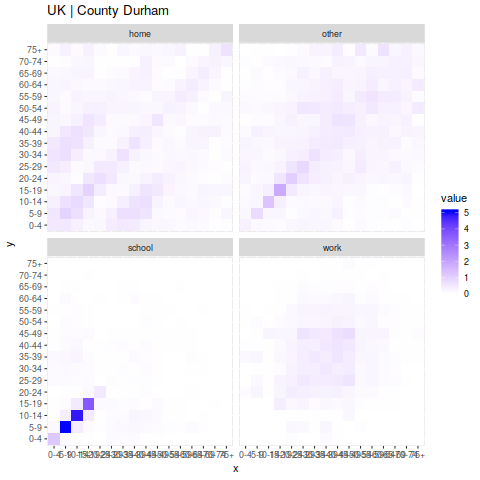
\includegraphics[width=.9\linewidth]{1-home-parameters.png}
\end{center}

Split matrices.

Second parameter is bounds, set to index of ``70-74''. Two
matrices formed from contact values of ``70-74'' and above (inclusive), and
``65-69'' and below. This is done for every population.
Only contact matrices are affected.
\begin{minted}[bgColor=LightGray]{r}
parameters = cm_split_matrices_ex_in(parameters, 15);
\end{minted}

Matrices for first population again:
\begin{center}
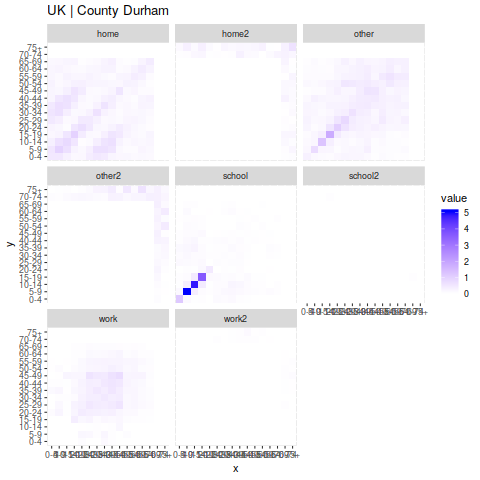
\includegraphics[width=.9\linewidth]{1-home-parameters-after-split.png}
\end{center}

For each population (i.e. region), we add a new matrix ``gran'',
for child-grandparent contacts.

mat\textsubscript{ref} is formed from total of home, other, home2 and other2 (essentially total
of home and other, for all ages).

This only does anything for analysis = 4.
Otherwise, it's an matrix of zeros.

For analysis for, it assumes that all (or a constant portion) of the time of
grandparents is spent with children.

For age 0-4, grandparents are everyone above 55
For age 5-9, grandparents are everyone above 60
For age 10-14, grandparents are everyone above 65
\begin{minted}[bgColor=LightGray]{r}
# Create child-elderly contacts

# Create additional matrix for child-elderly contacts
for (j in seq_along(parameters$pop))
{
  # Recover home/other contact matrix
  mat_ref <- parameters$pop[[j]]$matrices[[1]] + parameters$pop[[j]]$matrices[[4]] +
    parameters$pop[[j]]$matrices[[5]] + parameters$pop[[j]]$matrices[[8]]

  gran <- 5 / 7 # adjustment for weekdays only.
  N <- nrow(mat_ref)
  popsize <- parameters$pop[[j]]$size
  mat <- matrix(0, ncol = N, nrow = N)

  # Add child-grandparent contacts: under 15s to 55+s
  if (analysis == 4) {
    for (a in 1:3) {
      # pick out only contact between above 55, then 60, then 64 and child
      dist <- c(rep(0, 10 + a), mat_ref[a, (11 + a):N])
      # re-normalise (total = 1)
      dist <- dist / sum(dist)
      mat[a, ] <- mat[a, ] + gran * dist
      mat[, a] <- mat[, a] + (gran * dist) * (popsize[a] / popsize)
    }
  }

  # Add child-grandparent contact matrix to population
  parameters$pop[[j]]$matrices$gran <- mat
  parameters$pop[[j]]$contact <- c(parameters$pop[[j]]$contact, 0)
}
\end{minted}

For entry \#4 the gran matrix looks like this:
This is related to dist of contact of 

\begin{center}
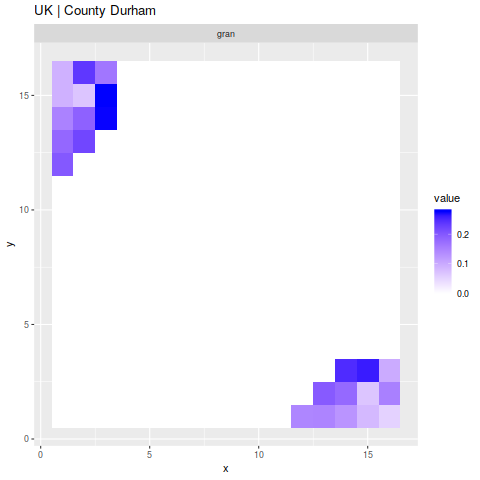
\includegraphics[width=.9\linewidth]{1-home-parameters-after-split-and-gran.png}
\end{center}

\begin{center}
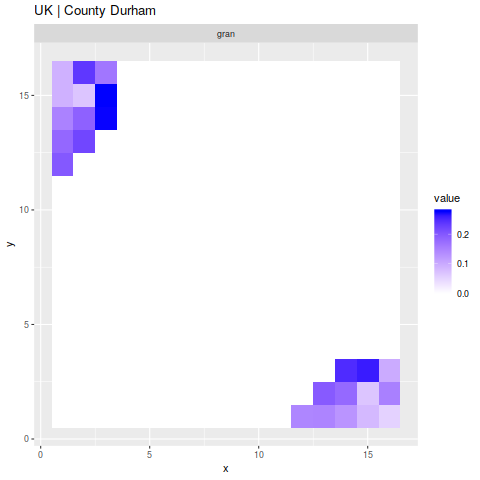
\includegraphics[width=.9\linewidth]{1-home-parameters-after-split-and-gran.png}
\end{center}

Read probs variable. I presume this to be the probability of individuals in
various age ranges who contract (?) the virus of being in various states
relevant to the health system.

\begin{minted}[bgColor=LightGray]{r}
# Health burden processes
probs = fread(
"Age,Prop_symptomatic,IFR,Prop_inf_hosp,Prop_inf_critical,Prop_critical_fatal,Prop_noncritical_fatal,Prop_symp_hospitalised,Prop_hospitalised_critical
10,0.66,8.59E-05,0.002361009,6.44E-05,0.5,0,0,0.3
20,0.66,0.000122561,0.003370421,9.19E-05,0.5,9.47E-04,0.007615301,0.3
30,0.66,0.000382331,0.010514103,0.000286748,0.5,0.001005803,0.008086654,0.3
40,0.66,0.000851765,0.023423527,0.000638823,0.5,0.001231579,0.009901895,0.3
50,0.66,0.001489873,0.0394717,0.001117404,0.5,0.002305449,0.018535807,0.3
60,0.66,0.006933589,0.098113786,0.005200192,0.5,0.006754596,0.054306954,0.3
70,0.66,0.022120421,0.224965092,0.016590316,0.5,0.018720727,0.150514645,0.3
80,0.66,0.059223786,0.362002579,0.04441784,0.5,0.041408882,0.332927412,0.3
100,0.66,0.087585558,0.437927788,0.065689168,0.5,0.076818182,0.617618182,0.3")
\end{minted}

\begin{minted}[bgColor=LightGray]{org}
10	0.66	8.59e-05	0.002361009	6.44e-05	0.5	0	0	0.3
20	0.66	0.000122561	0.003370421	9.19e-05	0.5	0.000947	0.007615301	0.3
30	0.66	0.000382331	0.010514103	0.000286748	0.5	0.001005803	0.008086654	0.3
40	0.66	0.000851765	0.023423527	0.000638823	0.5	0.001231579	0.009901895	0.3
50	0.66	0.001489873	0.0394717	0.001117404	0.5	0.002305449	0.018535807	0.3
60	0.66	0.006933589	0.098113786	0.005200192	0.5	0.006754596	0.054306954	0.3
70	0.66	0.022120421	0.224965092	0.016590316	0.5	0.018720727	0.150514645	0.3
80	0.66	0.059223786	0.362002579	0.04441784	0.5	0.041408882	0.332927412	0.3
100	0.66	0.087585558	0.437927788	0.065689168	0.5	0.076818182	0.617618182	0.3
\end{minted}

Names
\begin{minted}[bgColor=LightGray]{r}
probs
\end{minted}

\begin{minted}[bgColor=LightGray]{org}

   Age Prop_symptomatic         IFR Prop_inf_hosp Prop_inf_critical Prop_critical_fatal Prop_noncritical_fatal Prop_symp_hospitalised Prop_hospitalised_critical
1:  10             0.66 0.000085900   0.002361009       0.000064400                 0.5            0.000000000            0.000000000                        0.3
2:  20             0.66 0.000122561   0.003370421       0.000091900                 0.5            0.000947000            0.007615301                        0.3
3:  30             0.66 0.000382331   0.010514103       0.000286748                 0.5            0.001005803            0.008086654                        0.3
4:  40             0.66 0.000851765   0.023423527       0.000638823                 0.5            0.001231579            0.009901895                        0.3
5:  50             0.66 0.001489873   0.039471700       0.001117404                 0.5            0.002305449            0.018535807                        0.3
6:  60             0.66 0.006933589   0.098113786       0.005200192                 0.5            0.006754596            0.054306954                        0.3
7:  70             0.66 0.022120421   0.224965092       0.016590316                 0.5            0.018720727            0.150514645                        0.3
8:  80             0.66 0.059223786   0.362002579       0.044417840                 0.5            0.041408882            0.332927412                        0.3
9: 100             0.66 0.087585558   0.437927788       0.065689168                 0.5            0.076818182            0.617618182                        0.3
\end{minted}


Reformat probabilities:
\begin{minted}[bgColor=LightGray]{r}

reformat = function(P)
{
    # 70-74,3388.488  75-79,2442.147  80-84,1736.567  85-89,1077.555  90-94,490.577  95-99,130.083  100+,15.834
    x = c(P[1:7], weighted.mean(c(P[8], P[9]), c(3388.488 + 2442.147, 1736.567 + 1077.555 + 490.577 + 130.083 + 15.834)));
    return (rep(x, each = 2))
}

P.icu_symp     = reformat(probs[, Prop_symp_hospitalised * Prop_hospitalised_critical]);
P.nonicu_symp  = reformat(probs[, Prop_symp_hospitalised * (1 - Prop_hospitalised_critical)]);
P.death_icu    = reformat(probs[, Prop_critical_fatal]);
P.death_nonicu = reformat(probs[, Prop_noncritical_fatal]);
hfr = probs[, Prop_noncritical_fatal / Prop_symp_hospitalised]


burden_processes = list(
    list(source = "Ip", type = "multinomial", names = c("to_icu", "to_nonicu", "null"), report = c("", "", ""),
        prob = matrix(c(P.icu_symp, P.nonicu_symp, 1 - P.icu_symp - P.nonicu_symp), nrow = 3, ncol = 16, byrow = T),
        delays = matrix(c(cm_delay_gamma(7, 7, 60, 0.25)$p, cm_delay_gamma(7, 7, 60, 0.25)$p, cm_delay_skip(60, 0.25)$p), nrow = 3, byrow = T)),

    list(source = "to_icu", type = "multinomial", names = "icu", report = "p",
        prob = matrix(1, nrow = 1, ncol = 16, byrow = T),
        delays = matrix(cm_delay_gamma(10, 10, 60, 0.25)$p, nrow = 1, byrow = T)),

    list(source = "to_nonicu", type = "multinomial", names = "nonicu", report = "p",
        prob = matrix(1, nrow = 1, ncol = 16, byrow = T),
        delays = matrix(cm_delay_gamma(8, 8, 60, 0.25)$p, nrow = 1, byrow = T)),

    list(source = "Ip", type = "multinomial", names = c("death", "null"), report = c("o", ""),
        prob = matrix(c(P.death_nonicu, 1 - P.death_nonicu), nrow = 2, ncol = 16, byrow = T),
        delays = matrix(c(cm_delay_gamma(22, 22, 60, 0.25)$p, cm_delay_skip(60, 0.25)$p), nrow = 2, byrow = T))
)
parameters$processes = burden_processes
str(burden_processes)
\end{minted}

\begin{minted}[bgColor=LightGray]{org}

List of 4
 $ :List of 6
  ..$ source: chr "Ip"
  ..$ type  : chr "multinomial"
  ..$ names : chr [1:3] "to_icu" "to_nonicu" "null"
  ..$ report: chr [1:3] "" "" ""
  ..$ prob  : num [1:3, 1:16] 0 0 1 0 0 ...
  ..$ delays: num [1:3, 1:241] 8.48e-11 8.48e-11 1.00 1.49e-07 1.49e-07 ...
 $ :List of 6
  ..$ source: chr "to_icu"
  ..$ type  : chr "multinomial"
  ..$ names : chr "icu"
  ..$ report: chr "p"
  ..$ prob  : num [1, 1:16] 1 1 1 1 1 1 1 1 1 1 ...
  ..$ delays: num [1, 1:241] 2.29e-16 1.08e-11 1.41e-09 3.14e-08 2.90e-07 ...
 $ :List of 6
  ..$ source: chr "to_nonicu"
  ..$ type  : chr "multinomial"
  ..$ names : chr "nonicu"
  ..$ report: chr "p"
  ..$ prob  : num [1, 1:16] 1 1 1 1 1 1 1 1 1 1 ...
  ..$ delays: num [1, 1:241] 1.32e-12 6.95e-09 3.25e-07 3.60e-06 1.96e-05 ...
 $ :List of 6
  ..$ source: chr "Ip"
  ..$ type  : chr "multinomial"
  ..$ names : chr [1:2] "death" "null"
  ..$ report: chr [1:2] "o" ""
  ..$ prob  : num [1:2, 1:16] 0 1 0 1 0.000947 ...
  ..$ delays: num [1:2, 1:241] 1.07e-41 1.00 2.64e-31 0.00 1.58e-26 ...
\end{minted}

Appear unused
\begin{minted}[bgColor=LightGray]{r}
clt_i = 1;
clt_n = 0;
\end{minted}

Define observer lockdown triggers
\begin{minted}[bgColor=LightGray]{r}
# Observer for lockdown scenarios
observer_lockdown = function(lockdown_trigger) function(time, dynamics)
{
    # Get current icu prevalence
    icu_prevalence = dynamics[t == time, sum(icu_p)];

    # Determine lockdown trigger
    trigger = lockdown_trigger;

    # If ICU prevalence exceeds a threshold, turn on lockdown
    if (icu_prevalence >= trigger) {
        return (list(csv = paste(time, "trace_lockdown", "All", 2, sep = ","),
            changes = list(contact_lowerto = c(1, 0.1, 0.1, 0.1,  1, 0.1, 0.1, 0.1,  1))));
    } else  {
        return (list(csv = paste(time, "trace_lockdown", "All", 1, sep = ","),
            changes = list(contact_lowerto = c(1, 1, 1, 1, 1, 1, 1, 1, 1))));
    }
    return (list(csv = paste(time, "trace_lockdown", "All", 1, sep = ",")))
}
\end{minted}

Not sure what this is. Pool for sampling initial condition?
\begin{minted}[bgColor=LightGray]{r}
covid_scenario = qread(file.path(covid_uk_path, "data/2-linelist_symp_fit_fIa0.5.qs"));
str(covid_scenario)
\end{minted}

\begin{minted}[bgColor=LightGray]{org}

Classes ‘data.table’ and 'data.frame':	18000 obs. of  13 variables:
 $ trial: int  0 0 0 0 0 0 0 0 0 0 ...
 $ lp   : num  -2398 -2399 -2398 -2399 -2398 ...
 $ chain: int  0 1 2 3 4 5 6 7 8 9 ...
 $ ll   : num  -2393 -2394 -2393 -2395 -2393 ...
 $ f_00 : num  0.125 0.105 0.117 0.139 0.122 ...
 $ f_10 : num  0.073 0.0576 0.0661 0.0608 0.0669 ...
 $ f_20 : num  0.308 0.25 0.253 0.273 0.286 ...
 $ f_30 : num  0.419 0.362 0.395 0.424 0.42 ...
 $ f_40 : num  0.444 0.395 0.407 0.403 0.428 ...
 $ f_50 : num  0.527 0.46 0.484 0.523 0.522 ...
 $ f_60 : num  0.774 0.658 0.771 0.725 0.781 ...
 $ f_70 : num  0.733 0.632 0.664 0.707 0.708 ...
 $ size : num  49.4 47.3 53.1 55.4 45.5 ...
 - attr(*, ".internal.selfref")=<
\end{minted}


Boolean flags for region/classification:
\begin{minted}[bgColor=LightGray]{r}
# Identify London boroughs for early seeding, and regions of each country for time courses
london = cm_structure_UK[match(str_sub(locations, 6), Name), Geography1 %like% "London"]
england = cm_structure_UK[match(str_sub(locations, 6), Name), Code %like% "^E" & !(Geography1 %like% "London")]
wales = cm_structure_UK[match(str_sub(locations, 6), Name), Code %like% "^W"]
scotland = cm_structure_UK[match(str_sub(locations, 6), Name), Code %like% "^S"]
nireland = cm_structure_UK[match(str_sub(locations, 6), Name), Code %like% "^N"]
westmid = cm_structure_UK[match(str_sub(locations, 6), Name), Name == "West Midlands (Met County)"]
cumbria = cm_structure_UK[match(str_sub(locations, 6), Name), Name == "Cumbria"]
\end{minted}

cm\textsubscript{structure}\textsubscript{UK} is read from a datafile (structure\textsubscript{UK.rds}).
Boolean flags for classification are derived by pattern matching on the file.
The cm\textsubscript{structure}\textsubscript{UK} is shown below. Presumably this is providing age distribution info.
\begin{verbatim}
Classes ‘data.table’ and 'data.frame':	430 obs. of  95 variables:
 $ Code      : chr  "K02000001" "K03000001" "K04000001" "E92000001" "E12000001" "E06000047" "E06000005" ...
 $ Name      : chr  "UNITED KINGDOM" "GREAT BRITAIN" "ENGLAND AND WALES" "ENGLAND" "NORTH EAST" "County Durham" "Darlington" ...
 $ Geography1: chr  "Country" "Country" "Country" "Country" "Region" "Unitary Authority" "Unitary Authority" ...
 $ All ages  : num  66435550 64553909 59115809 55977178 2657909 526980 106566 93242 140545 ...
 $ 0         : num  745263 722107 669797 637834 27275 4989 1134 999 1871 ...
 $ 1         : num  770614 746644 692792 659890 28355 5252 1104 1011 1970 ...
 $ 2         : num  796314 771397 715313 681032 29293 5448 1207 1101 1882 ...
 $ 3         : num  797183 772403 715338 680758 29138 5547 1216 1060 1969 ...
 $ 4         : num  804654 779741 722190 687213 30008 5785 1256 1126 1965 ...
 $ 5         : num  823204 797905 739193 703391 30795 5939 1314 1136 2025 ...
 $ 6         : num  848681 822531 762279 725210 31781 5929 1369 1200 1955 ...
 $ 7         : num  836008 810047 747953 710174 31880 6223 1284 1219 1975 ...
 $ 8         : num  819824 794129 734922 697777 31362 6140 1341 1218 1911 ...
 $ 9         : num  810807 784797 723973 687314 30492 5758 1342 1184 1740 ...
 $ 10        : num  816988 790978 730400 693071 31024 6065 1302 1182 1800 ...
 $ 11        : num  790130 765321 707081 671108 30014 5839 1284 1174 1741 ...
 $ 12        : num  774368 750726 693698 658113 30122 5801 1329 1148 1788 ...
 $ 13        : num  744924 721854 665305 630959 28377 5556 1225 1078 1636 ...
 $ 14        : num  732484 709693 654298 620868 27826 5297 1270 1018 1614 ...
 $ 15        : num  712733 690396 636635 603746 27256 5265 1203 1039 1521 ...
  [list output truncated]
 - attr(*, ".internal.selfref")=<externalptr>
\end{verbatim}

Columns for from 0-100.

\subsection{Aggregate function}
\label{sec:org61e6d37}
\subsubsection{Collect functions}
\label{sec:org4a84d18}

Two functions that are used later to aggregate results.

\begin{minted}[bgColor=LightGray]{r}
add_totals = function(run, totals)
{
    regions = run$dynamics[, unique(population)];

    # totals by age
    totals0 = run$dynamics[, .(total = sum(value)), by = .(scenario, run, compartment, group)];
    return (rbind(totals, totals0))
}

add_dynamics = function(run, dynamics, iv)
{
    regions = run$dynamics[, unique(population)];

    interv = data.table(scenario = run$dynamics$scenario[1], run = run$dynamics$run[1], t = unique(run$dynamics$t),
        compartment = "trace_school", region = "All", value = unlist(iv$trace_school));
    if (!is.null(iv$trace_intervention)) {
        interv = rbind(interv,
            data.table(scenario = run$dynamics$scenario[1], run = run$dynamics$run[1], t = unique(run$dynamics$t),
                compartment = "trace_intervention", region = "All", value = unlist(iv$trace_intervention)));
    } else {
        interv = rbind(interv,
            data.table(scenario = run$dynamics$scenario[1], run = run$dynamics$run[1], t = unique(run$dynamics$t),
                compartment = "trace_intervention", region = "All", value = 1));
    }

    csvlines = NULL;
    if (nchar(run$csv[[1]]) > 0) {
        csvlines = fread(run$csv[[1]], header = F);
        csvlines = cbind(run$dynamics$scenario[1], run$dynamics$run[1], csvlines);
        names(csvlines) = c("scenario", "run", "t", "compartment", "region", "value");
        csvlines = unique(csvlines);
    }

    # time courses
    return (rbind(dynamics,
        run$dynamics[population %in% locations[westmid],  .(region = "West Midlands",    value = sum(value)), by = .(scenario, run, t, compartment)],
        run$dynamics[population %in% locations[cumbria],  .(region = "Cumbria",          value = sum(value)), by = .(scenario, run, t, compartment)],
        run$dynamics[population %in% locations[london],   .(region = "London",           value = sum(value)), by = .(scenario, run, t, compartment)],
        run$dynamics[population %in% locations[england],  .(region = "England",          value = sum(value)), by = .(scenario, run, t, compartment)],
        run$dynamics[population %in% locations[wales],    .(region = "Wales",            value = sum(value)), by = .(scenario, run, t, compartment)],
        run$dynamics[population %in% locations[scotland], .(region = "Scotland",         value = sum(value)), by = .(scenario, run, t, compartment)],
        run$dynamics[population %in% locations[nireland], .(region = "Northern Ireland", value = sum(value)), by = .(scenario, run, t, compartment)],
        run$dynamics[,                                    .(region = "United Kingdom",   value = sum(value)), by = .(scenario, run, t, compartment)],
        interv,
        csvlines
    ))
}
\end{minted}
\section{Main}
\label{sec:org89244d4}
Define school terms (base vs intervention)
\begin{minted}[bgColor=LightGray]{r}
school_close_b =  c("2020-2-16", "2020-4-05", "2020-5-24", "2020-7-22", "2020-10-25", "2020-12-20", "2021-02-14", "2021-04-01", "2021-05-30", "2021-07-25");
school_reopen_b = c("2020-2-22", "2020-4-18", "2020-5-30", "2020-9-01", "2020-10-31", "2021-01-02", "2021-02-20", "2021-04-17", "2021-06-05", "2021-09-01");
school_close_i =  c("2020-2-16", "2020-4-05", "2020-5-24", "2020-7-22", "2020-10-25", "2020-12-20", "2021-02-14", "2021-04-01", "2021-05-30", "2021-07-25");
school_reopen_i = c("2020-2-22", "2020-4-18", "2020-5-30", "2020-9-01", "2020-10-31", "2021-01-02", "2021-02-20", "2021-04-17", "2021-06-05", "2021-09-01");
\end{minted}

Define some interventions, by their ``contact''. There are 9 groups here.
\begin{minted}[bgColor=LightGray]{r}
interventions = list(
    `School Closures`   = list(contact = c(1.0, 1.0, 0.0, 1.0,  1.0, 1.0, 0.0, 1.0,  0))
);
\end{minted}

Set the options
\begin{minted}[bgColor=LightGray]{r}
# should the lockdown be triggered nationally (in one go) or locally by region
option.trigger = "national";

# How long should the intervention last for?
option.duration = 7 * 12;

# Is this a lockdown?
option.lockdown = NA;

# Allows to intervention wrt to computed peak of infection
# 0 is centered at peak.
option.intervention_shift = 0;
\end{minted}

Pick R0 from a normal distribution.
\begin{minted}[bgColor=LightGray]{r}
set.seed(9876);
R0s = rnorm(n_runs, mean = 2.675739, sd = 0.5719293)
\end{minted}

\begin{minted}[bgColor=LightGray]{org}
3.26044660116393
2.01494818798272
2.56678063560151
2.62267317062699
2.68651581109931
\end{minted}

Set up some empty aggregate data structures
\begin{minted}[bgColor=LightGray]{r}
dynamics = data.table()
totals = data.table()
print(Sys.time())
set.seed(1234567);
\end{minted}

Seed again
\begin{minted}[bgColor=LightGray]{r}
set.seed(1234567);
\end{minted}
\section{Start Runs}
\label{sec:org669d344}
\begin{itemize}
\item Note taken on \textit{[2020-05-18 Mon 00:08]}
\end{itemize}
Set an R0 (this happens in the loop)
\begin{minted}[bgColor=LightGray]{r}
r = R0s[1]
\end{minted}

\begin{minted}[bgColor=LightGray]{org}
3.26044660116393
\end{minted}

\begin{minted}[bgColor=LightGray]{r}
covid_scenario
\end{minted}

\begin{minted}[bgColor=LightGray]{org}

       trial        lp chain        ll      f_00       f_10      f_20      f_30      f_40      f_50      f_60      f_70     size
    1:     0 -2397.630     0 -2392.980 0.1247845 0.07295634 0.3075943 0.4191281 0.4439132 0.5273762 0.7743843 0.7325784 49.40969
    2:     0 -2398.569     1 -2393.768 0.1051005 0.05757648 0.2498489 0.3619066 0.3948041 0.4599669 0.6578147 0.6319850 47.29300
    3:     0 -2397.795     2 -2392.965 0.1174401 0.06606591 0.2525465 0.3949755 0.4074855 0.4836499 0.7707342 0.6637128 53.07236
    4:     0 -2399.340     3 -2394.679 0.1391260 0.06079020 0.2734493 0.4237577 0.4026213 0.5227978 0.7247470 0.7069094 55.40430
    5:     0 -2397.630     4 -2392.885 0.1221617 0.06693948 0.2855716 0.4199246 0.4280588 0.5219734 0.7810006 0.7075087 45.52440
   ---                                                                                                                          
17996:   999 -2397.475    13 -2392.335 0.1570445 0.09094176 0.3294248 0.4943820 0.4901900 0.6161672 0.8954522 0.8188619 50.36484
17997:   999 -2399.101    14 -2394.203 0.1229701 0.05235644 0.2418619 0.3549702 0.3897229 0.4407649 0.6885768 0.6358008 56.79066
17998:   999 -2398.274    15 -2392.305 0.1672379 0.08747932 0.3686038 0.4616906 0.5003443 0.6532227 0.9553297 0.8344203 48.53948
17999:   999 -2399.586    16 -2395.207 0.1368256 0.07047143 0.3017713 0.3947725 0.4164846 0.5487908 0.7288546 0.6672768 43.46868
18000:   999 -2398.206    17 -2393.266 0.1318261 0.05292663 0.2455728 0.3296847 0.3494939 0.4654164 0.7121425 0.6454375 55.55304
\end{minted}

Unifromly sample a ``scenario'' (age-varying symptomatic rate, apparently).
This is just a row in the covid\textsubscript{scenario} table, which was data.
\begin{minted}[bgColor=LightGray]{r}
# 1. Pick age-varying symptomatic rate
covy = unname(unlist(covid_scenario[sample.int(nrow(covid_scenario), 1), f_00:f_70]));
covy = rep(covy, each = 2);
\end{minted}

Set UK scenario ``y'' to covy (avsr)
\begin{minted}[bgColor=LightGray]{r}
parametersUK1$pop[[1]]$y = covy;
\end{minted}

\begin{minted}[bgColor=LightGray]{org}
0.110365454000957
0.110365454000957
0.0658313431091681
0.0658313431091681
0.267296120911696
0.267296120911696
0.411541875601079
0.411541875601079
0.390821035209271
0.390821035209271
0.515082503370863
0.515082503370863
0.697017073733944
0.697017073733944
0.615829335365191
0.615829335365191
\end{minted}

Calculate an adjustment (a number)
\begin{minted}[bgColor=LightGray]{r}
cm_calc_R0(parametersUK1, 1);
\end{minted}

\begin{minted}[bgColor=LightGray]{org}
3.13591243385139
\end{minted}

Compute u\textsubscript{adj} (numeric)
\begin{minted}[bgColor=LightGray]{r}
u_adj = r / cm_calc_R0(parametersUK1, 1);
\end{minted}

\begin{minted}[bgColor=LightGray]{org}
1.0397122591716
\end{minted}

Pick seeding times
\begin{minted}[bgColor=LightGray]{r}
seed_start = ifelse(london, sample(0:6, length(london), replace = T), sample(0:20, length(london), replace = T));
\end{minted}

\begin{minted}[bgColor=LightGray]{org}
 int [1:186] 1 15 6 1 16 15 17 2 17 7 ...
\end{minted}

Set parameters (u\textsubscript{adj}, covy, seed\textsubscript{times}). Compute dist\textsubscript{seed}\textsubscript{ages}
\begin{minted}[bgColor=LightGray]{r}
    params = duplicate(parameters);
    for (j in seq_along(params$pop)) {
        params$pop[[j]]$u = params$pop[[j]]$u * u_adj;
        params$pop[[j]]$y = covy;
        params$pop[[j]]$seed_times = rep(seed_start[j] + 0:27, each = 2);
        params$pop[[j]]$dist_seed_ages = cm_age_coefficients(25, 50, 5 * 0:16);
    }
\end{minted}

\begin{minted}[bgColor=LightGray]{r}
params$pop[[1]]$seed_times
\end{minted}

\begin{minted}[bgColor=LightGray]{org}
 [1]  9  9 10 10 11 11 12 12 13 13 14 14 15 15 16 16 17 17 18 18 19 19 20 20 21 21 22 22 23 23 24 24 25 25 26 26 27 27 28 28 29 29 30 30 31 31 32 32 33 33 34 34 35 35 36 36
\end{minted}

Ages seed appears deterministic
\begin{minted}[bgColor=LightGray]{r}
params$pop[[1]]$dist_seed_ages
\end{minted}

\begin{minted}[bgColor=LightGray]{org}
 [1] 0 0 0 0 0 1 1 1 1 1 0 0 0 0 0 0
\end{minted}

Set school terms
\begin{minted}[bgColor=LightGray]{r}
    # 4b. Set school terms
    iv = cm_iv_build(params)
    cm_iv_set(iv, school_close_b, school_reopen_b, contact = c(1, 1, 0, 1,  1, 1, 0, 1,  1), trace_school = 2);
    params = cm_iv_apply(params, iv);
\end{minted}


Parameters for simulation:
\begin{minted}[bgColor=LightGray]{r}
print_params(params, 10)
\end{minted}

\begin{minted}[bgColor=LightGray]{org}
Duration fields:
 date0 : 2020-01-29
 time0 : 0
 time1 : 2021-12-31
 time_step : 0.25


Behavioural flag fields
 fast_multinomial : NA
 deterministric : NA


Populations [186]:
UK | County Durham
UK | Darlington
UK | Hartlepool
UK | Middlesbrough
UK | Northumberland
UK | Redcar and Cleveland
UK | Stockton-on-Tees
UK | Tyne and Wear (Met County)
UK | Blackburn with Darwen
UK | Blackpool ...
\end{minted}

Population fields:
\begin{minted}[bgColor=LightGray]{r}
print_population_fields(params)
\end{minted}

\begin{minted}[bgColor=LightGray]{org}
  time_step       : num 0.25
  date0           : chr "2020-01-29"
  time0           : num 0
  time1           : chr "2021-12-31"
  report_every    : num 4
  fast_multinomial: logi FALSE
  deterministic   : logi FALSE
  pop             :List of 186
  travel          : num [1:186, 1:186] 1 0 0 0 0 0 0 0 0 0 ...
  processes       :List of 4
\end{minted}

Contact Matrices:
\begin{minted}[bgColor=LightGray]{r}
plot_matrices(params$pop[[1]])
\end{minted}

\begin{center}
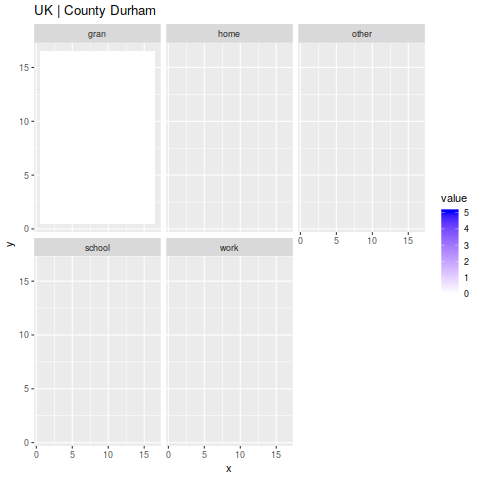
\includegraphics[width=.9\linewidth]{1-intervention-all.png}
\end{center}

\begin{minted}[bgColor=LightGray]{r}
# run = cm_simulate(params, 1, 1);
run$dynamics[, run := r];
run$dynamics[, scenario := "Base"];
run$dynamics[, R0 := R0s[1]];
\end{minted}

\begin{minted}[bgColor=LightGray]{org}
Error in ymd(t) : could not find function "ymd"

Error: object 'run' not found

Error: object 'run' not found

Error: object 'run' not found
\end{minted}
\end{document}
